%%%%%%%%%%%%%%%%%%%%%%%%%%%%%%%%%%%%%%%%%%%%%%%%%%%
%% LaTeX book template                           %%
%% Author:  Amber Jain (http://amberj.devio.us/) %%
%% License: ISC license                          %%
%%%%%%%%%%%%%%%%%%%%%%%%%%%%%%%%%%%%%%%%%%%%%%%%%%%

\documentclass[a4paper,11pt]{book}
\usepackage[T1]{fontenc}
\usepackage[utf8]{inputenc}
\usepackage{lmodern}
%%%%%%%%%%%%%%%%%%%%%%%%%%%%%%%%%%%%%%%%%%%%%%%%%%%%%%%%%
% Source: http://en.wikibooks.org/wiki/LaTeX/Hyperlinks %
%%%%%%%%%%%%%%%%%%%%%%%%%%%%%%%%%%%%%%%%%%%%%%%%%%%%%%%%%
\usepackage{hyperref}
\usepackage{graphicx}
\usepackage[english]{babel}

%%%%%%%%%%%%%%%%%%%%%%%%%%%%%%%%%%%%%%%%%%%%%%%%%%%%%%%%%%%%%%%%%%%%%%%%%%%%%%%%
% 'dedication' environment: To add a dedication paragraph at the start of book %
% Source: http://www.tug.org/pipermail/texhax/2010-June/015184.html            %
%%%%%%%%%%%%%%%%%%%%%%%%%%%%%%%%%%%%%%%%%%%%%%%%%%%%%%%%%%%%%%%%%%%%%%%%%%%%%%%%
\newenvironment{dedication}
{
   \cleardoublepage
   \thispagestyle{empty}
   \vspace*{\stretch{1}}
   \hfill\begin{minipage}[t]{0.66\textwidth}
   \raggedright
}
{
   \end{minipage}
   \vspace*{\stretch{3}}
   \clearpage
}

%%%%%%%%%%%%%%%%%%%%%%%%%%%%%%%%%%%%%%%%%%%%%%%%
% Chapter quote at the start of chapter        %
% Source: http://tex.stackexchange.com/a/53380 %
%%%%%%%%%%%%%%%%%%%%%%%%%%%%%%%%%%%%%%%%%%%%%%%%
\makeatletter
\renewcommand{\@chapapp}{}% Not necessary...
\newenvironment{chapquote}[2][2em]
  {\setlength{\@tempdima}{#1}%
   \def\chapquote@author{#2}%
   \parshape 1 \@tempdima \dimexpr\textwidth-2\@tempdima\relax%
   \itshape}
  {\par\normalfont\hfill--\ \chapquote@author\hspace*{\@tempdima}\par\bigskip}
\makeatother

%%%%%%%%%%%%%%%%%%%%%%%%%%%%%%%%%%%%%%%%%%%%%%%%%%%
% First page of book which contains 'stuff' like: %
%  - Book title, subtitle                         %
%  - Book author name                             %
%%%%%%%%%%%%%%%%%%%%%%%%%%%%%%%%%%%%%%%%%%%%%%%%%%%

% Book's title and subtitle
\title{\Huge \textbf{Electric Circuits}  \\ \huge An Introduction}
% Author
\author{Robert Brown \\ Darby Hewitt}


\begin{document}

\frontmatter
\maketitle

%%%%%%%%%%%%%%%%%%%%%%%%%%%%%%%%%%%%%%%%%%%%%%%%%%%%%%%%%%%%%%%
% Add a dedication paragraph to dedicate your book to someone %
%%%%%%%%%%%%%%%%%%%%%%%%%%%%%%%%%%%%%%%%%%%%%%%%%%%%%%%%%%%%%%%
\begin{dedication}
Dedicated to some cool people.
\end{dedication}

%%%%%%%%%%%%%%%%%%%%%%%%%%%%%%%%%%%%%%%%%%%%%%%%%%%%%%%%%%%%%%%%%%%%%%%%
% Auto-generated table of contents, list of figures and list of tables %
%%%%%%%%%%%%%%%%%%%%%%%%%%%%%%%%%%%%%%%%%%%%%%%%%%%%%%%%%%%%%%%%%%%%%%%%
\tableofcontents
%\listoffigures
%\listoftables

\mainmatter
\chapter*{Preface}
This book is made in reaction to many introductory Electrical Engineering texts, which tend to assume a Sophomore- or even Junior-level understanding of Mathematics.  In contrast, we aim our text at Freshmen, who may or may not have completed Calculus I.

%%%%%%%%%%%%%%%%%%%%%%%%%%%%%%%%%%%%
% Give credit where credit is due. %
% Say thanks!                      %
%%%%%%%%%%%%%%%%%%%%%%%%%%%%%%%%%%%%
\section*{Acknowledgements}
\begin{itemize}
\item To Robert and Darby, who are awesome!
\item To the students, who are awesome!
\item To circuits, which is awesome!
\end{itemize}

% ---------------------------------------------------------------------
\chapter{Underlying Fundamentals}
\section{Review of Algebra}
The things in this section are parts of mathematics that are critical to success in an introductory Circuits course, but that we assume you already know.  In that vein, this section will not be an in-depth coverage of the topic of Algebra, but rather an overview of the specific topics that you will need.
\subsection*{Isolating Variables}
\subsection*{Simple Systems of Equations}
\subsection*{Trigonometry}
\subsection*{Sine and Cosine Curves}


\section{Units}
\subsection{What is charge?}
\subsection{Current, Voltage, Resistance}

\section{A Word on Graphs}
The first thing you probably think of when you hear the word graph is plugging $y=mx+b$ into your calculator.  For the rest of this book, we'll refer to that concept as a plot.

A graph in a purely mathematical sense is a collection of {\bf nodes} and
{\bf branches}. Nodes are like locations or specific points in space, and
branches are the connections between the nodes (similar to pathways between the various locations).  You can draw a graph of this type as shown in Figure \ref{fig:graphTheory}.

% Figure of Example Graph
\begin{figure}
%  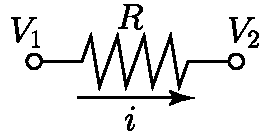
\includegraphics[width=0.5\linewidth]{figures/ohmsLaw}
  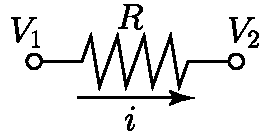
\includegraphics{figures/ohmsLaw}
  \caption{Pictured is a graph, which consists of a number of nodes and branches connecting those nodes.}
  \label{fig:graphTheory}
\end{figure}

We will be using the concept of a graph to talk about electric circuits.


\section{What is a Circuit?}

\section{Vector Mathematics}
\input{ch_prelim/vector_math}

\section{Complex Numbers}
\begin{itemize}
\item Complex numbers builds on our understanding of vectors
\item If all real numbers can be plotted on a number line, we can draw another number line orthogonal\footnote{perpendicular} to the first to represent imaginary numbers.  A complex number is a point within the plane we created.
\item Complex numbers can be represented in two ways: Cartesian form and polar form
  \begin{itemize}
  \item In Cartesian form, the real and imaginary parts are simply added together, with the imaginary part multiplied with $j$, which is the Circuits name for $\sqrt{\-1}$.  For instance, $1 + j2$ would be a number which is one unit to the right on the Real number line, and two units up on the imaginary number line.
  \item In polar form, a line connecting the point to the origin is defined, and the point is then described using the length of that line and the angle it makes with the Real number line.  $1 + j2$ would have a length of $\sqrt{5}$ and an angle of about 63 degrees or 1.1 rad.  This is commonly represented as $\sqrt{5}e^{j1.1}$ or just $\sqrt{5}\angle{1.1}$
  \item If a number $C$ can be described as $C=x+jy$, it can be converted to polar coordinates ($C=A\angle \theta$) through the following formulas:
    \begin{itemize}
    \item $A = \sqrt{x^2+y^2}$
    \item $\theta = \tan^{-1}\frac{y}{x}$
    \end{itemize}
  \item Likewise, the number can be converted back using these formulas:
    \begin{itemize}
    \item $x = A\cos \theta$
    \item $y = A\sin \theta$
    \end{itemize}
  \end{itemize}
\item Addition is only feasible in Cartesian coordinates.  If you need to add two imaginary numbers in polar form, you should convert both to Cartesian first.
  \begin{itemize}
  \item Take two complex numbers in Cartesian form: $C_1=x_1+jy_1$ and
    $C_2=x_2+jy_2$
  \item The sum of those two numbers is defined as
    $C_1+C_2=(x_1+x_2)+j(y_1+y_2)$
  \item To subtract $C_2$ from the $C_1$, simply negate both $x_2$ and $y_2$:
    $C_1-C_2=(x_1-x_2)+j(y_1-y_2)$
  \end{itemize}
\item Multiplication is feasible in either Cartesian or polar coordinates
  \begin{itemize}
  \item Take two complex numbers in Cartesian form: $C_1=x_1+jy_1$ and
    $C_2=x_2+jy_2$
  \item The product of those two can be written through the FOIL (First, Outer, Inner, Last) method: $C_1\cdot C_2 = x_1x_2 + jx_1y_2 + jx_2y_1 + j^2y_1y_2$
  \item Recognize that $j^2=-1$:
    $C_1\cdot C_2 = x_1x_2 + jx_1y_2 + jx_2y_1 - y_1y_2$
  \item Alternatively, if you have two complex numbers in polar form: $C_1=A_1\angle\theta_1$ and $C_2=A_2\angle\theta_2$
  \item The new amplitude is simply the product of the original amplitudes, and the new angle is the sum of the original angles:
    $C_1\cdot C_2 = C_1C_2\angle(\theta_1+\theta_2)$
  \end{itemize}
\item Division is possible in Cartesian coordinates, but difficult enough that it is much easier to simply convert to polar
  \begin{itemize}
  \item Take two numbers in polar form: $C_1=A_1\angle\theta_1$ and $C_2=A_2\angle\theta_2$
  \item The new amplitude is the result of the division of the original amplitudes, and the new angle is the result of subtraction of the original amplitudes: $C_1/C_2 = A_1/A_2 \angle(\theta_1 - \theta_2)$
  \end{itemize}
\end{itemize}


\section{Linear Algebra}
The first thing to note is that linear algebra is a huge subject with applications not only in circuit analysis, but also in artificial intelligence, simulation and modeling, signal analysis, and computer graphics, just to name a few.  We will only be scratching the surface by covering matrix/vector algebra and matrix inversion.
\subsection*{What is a Matrix?}
A matrix is simply a collection of numbers in an array of a specific size.
For instance, a 2x3 matrix could be written as follows:
\begin{equation*}
  A = \left[
    \begin{tabular}{ccc}
      2 & 1 & -4 \\
      $\pi$ & $2/9$ & 14
    \end{tabular}
    \right]
\end{equation*}
Note that the first number in the size refers to the width or the number of columns of the matrix.  The second refers to the height or the number of rows.

Vectors, by contrast, will always have one of their dimensions that has a length of 1.  A {\bf row vector} would have a size of Nx1, while a {\bf column vector} would have a size of 1xN.
\begin{align*}
  x_{row} =& \left\{\begin{tabular}{ccc} 20 & $\sqrt{2}$ & 0.2 \end{tabular}\right\} &
  x_{col} =& \left\{\begin{tabular}{c} 5 \\ $e^2$ \\ 2 \end{tabular}\right\}
\end{align*}

A {\bf scalar} is a normal number that we are used to working with.  It could be defined as a matrix with a size of 1x1.

\subsection*{Matrix/Vector Algebra}
%% Addition/Subtraction
Once we have some matrices and vectors defined, we can start performing some mathematical operations on them.  First, we have addition/subtraction.  The most important thing to note is that the matrices we use MUST have the same size for us to add or subtract them.  

%% Transpose
Since matrices and vectors have some size and shape to them, we have the ability to move around the numbers inside them.  The operator that does this is known as the {\bf transpose} operator.  Transposing the matrix $A$ from before results in:
\begin{equation*}
  A^T = \left[
    \begin{tabular}{cc}
      2 & $\pi$ \\
      1& $2/9$ \\
      -4 & 14
    \end{tabular}
    \right]
\end{equation*}
Looking at each column, the values come from the original rows.

%% Matrix Vector Multiplication
Multiplication is a bit trickier.  In order to multiply two matrices, the number of rows of the first matrix must match the number of columns for the second matrix.  Also, some of the normal rules of scalar multiplication ($a b = b a$) are slightly modified ($A B = B^T A$)

\subsection*{Writing Systems of Equations Using Linear Algebra}

\subsection*{Matrix Inversion}


\section{Computer Resources - Matlab}
\subsection{Setting up Matlab/Octave}
\subsection{Using Matlab to Solve Problems}
\section{Computer Resources - Python}
\subsection{Setting up Python}
\subsection{Using Python to Solve Problems}

%%%%%%%%%%%%%%%%%%%%%%%%%%%%%%
\part{DC Circuit Analysis}
%%%%%%%%%%%%%%%%%%%%%%%%%%%%%%

% --------------------------------------------------------------------
\chapter{The First Laws}

\section{Ohm's Law on a Single Resistor}

\section{Ohm's Law on a Simple Circuit}

\section{Kirchoff's Current Law}

\section{Watt's Law}

% --------------------------------------------------------------------
\chapter{Circuit Simplification and Re-Expansion}
\section{Resistors in Series}
\section{Resistors in Paralle}
\section{Reorganizing Complex Circuits}
\section{Using Voltage Division}
\section{Using Current Division}

% --------------------------------------------------------------------
\chapter{Extra Uses for Voltage Dividers}
\section{Maximum Power Transfer}

\section{Nonlinear Circuit Elements}

% --------------------------------------------------------------------
\chapter{Operational Amplifiers}
\section{What is an Op-Amp?}

\section{Golden Rules}

\section{Analyzing Circuits with Op-Amps}

%%%%%%%%%%%%%%%%%%%%%%%%%%%%%
\part{Alternating Current}
%%%%%%%%%%%%%%%%%%%%%%%%%%%%%

% --------------------------------------------------------------------
\chapter{AC Circuits}
\section{Phasor Notation}
\section{Capacitors}
\section{Inductors}
\section{Impedance and Ohm's Law}


% --------------------------------------------------------------------
\chapter{Passive Filters}
\section{Frequency Response}
\section{First Order Filters}
\section{Second Order Filters}

% --------------------------------------------------------------------
\chapter{Active Filters}
\section{Op-Amps in AC}
\section{First Order Filters}
\section{Second Order Filters}

%%%%%%%%%%%%%%%%%%%%%%%%%%%%%%%%%%%
\part{Analysis of Complex Circuits}
%%%%%%%%%%%%%%%%%%%%%%%%%%%%%%%%%%%
% --------------------------------------------------------------------
\chapter{Node Voltage Method}

\chapter{Mesh Current Method}


\end{document}
